\section{Einleitung}
In unserem Projekt zur Vorlesung ``Algorithmen für geografische Informationssysteme'' stellen wir das Problem der ``Viewshed''-Analyse vor und 
vergleichen verschiedene Lösungs-Algorithmen. \\ Der englische Begriff \textit{viewshed} ist definiert als \textit{die geografische Fläche, die 
von einem bestimmtem Standpunkt aus sichtbar ist}. Der viewshed wird beispielweise bei folgenden Problemstellungen benötigt:
\begin{itemize}
 \item Bestimmung günstiger Standorte für Sendemasten
 \item Finden von Aussichtspunkten (z.B. im Gebirge), um Wanderwege planen zu können
 \item Finden von versteckten Punkten (z.B. für militärische Zwecke)
 \item Finden von besonders schönen Routen, z.B. entlang der Küste 
\end{itemize}
\begin{figure}[!ht]
\begin{minipage}{0.45\textwidth}
\centering
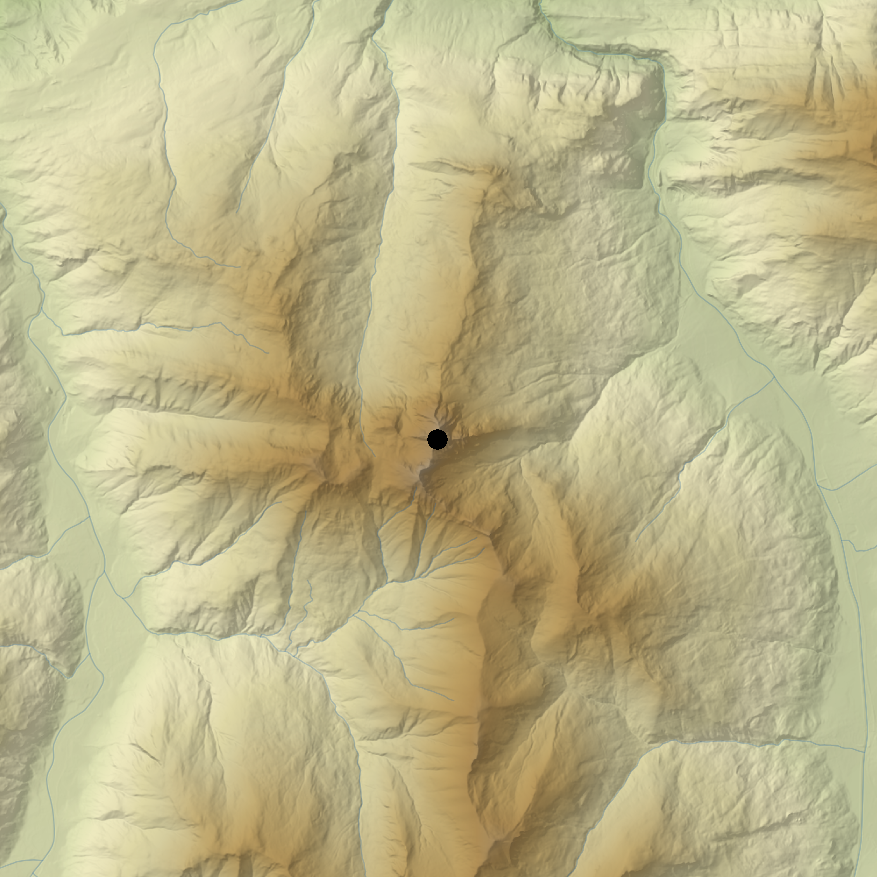
\includegraphics[scale=0.85]{bilder/berg_viewpoint}
\caption{Landkarte im Gebirge, der Standpunkt ist schwarz markiert}
\end{minipage}
\hfill
\begin{minipage}{0.45\textwidth}
\centering
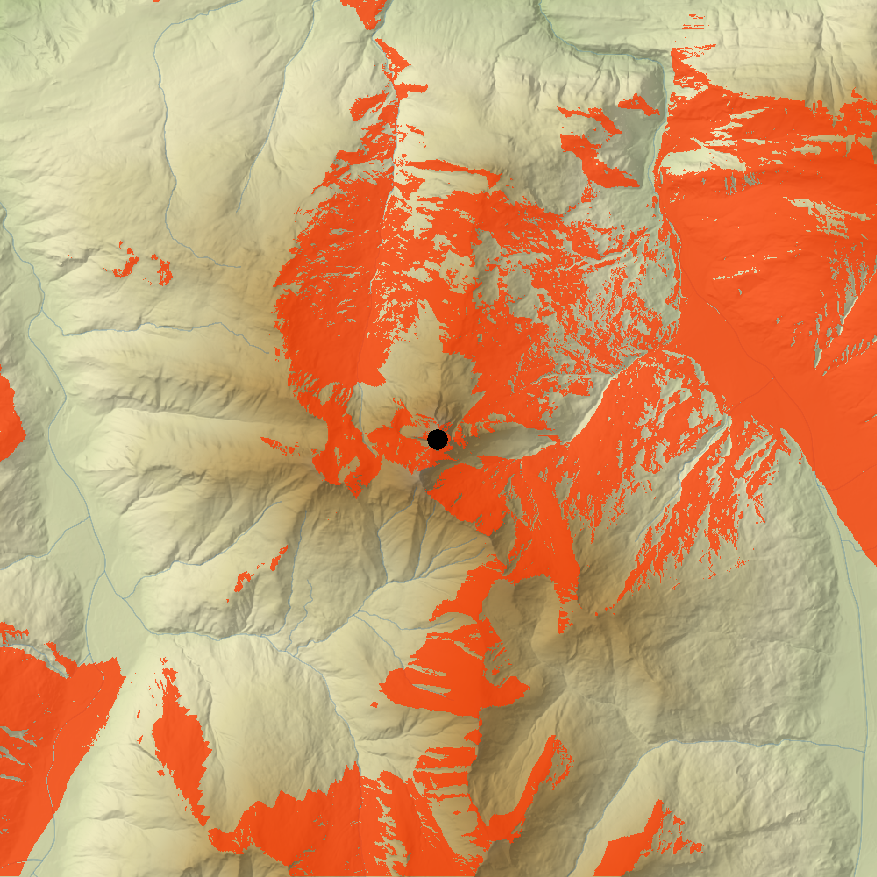
\includegraphics[scale=0.85]{bilder/berg_viewshed}
\caption{Die rote Fläche zeigt den vom Standpunkt aus sichtbaren Teil des Gebiets}
\end{minipage}
\end{figure}

Um den viewshed bestimmen zu können, ist ein sogenanntes \textit{digital elevation model} (DEM) nötig. 
Dieses digitale Höhenmodell ist eine Rasterkarte und enthält die Höhendaten des zugrunde liegenden Gebietes. 
Dargestellt wird das DEM als zweidimensionales Array, in dem die Höhendaten gespeichert sind. 

\noident Für die Berechnung des viewsheds wird neben dem Höhenmodell auch ein Standpunkt benötigt, von welchem ausgehend die Sichtbarkeit anderer Punkte bestimmt werden soll. 
Sofern der Standpunkt oberhalb des Bodenniveaus liegen soll (etwa für Sendemasten, Einbeziehung der Augenhöhe oä.) kann zusätzlich eine Höhenangabe angegeben werden. 

%\noindent Ein DEM ist eine zwei- oder dreidimensionale Darstellung einer geografischen Karte und enthält die Höhendaten des dargestellten Gebiets. 
%Für unsere Problemstellung ist die zweidimensionale Variante ausreichend.

%\noindent In einem DEM, welches als zweidimensionales Array dargestellt werden kann, wird ein Punkt als Standort gewählt. Um z.B. die Höhe eines 
%Sendemasten miteinzuberechnen, kann auch eine zusätzliche Höhe angegeben werden, welche auf die Höhe des Standorts addiert wird.

\noindent Als Testdaten wurden DEMs der Bayerischen Vermessungsverwaltung \cite{berchtesgaden} und des Salzburger Geographischen Informationssystems 
\cite{salzburg} verwendet. Da die Testdaten in einer simplen Textdatei im ASCII-Grid Format (siehe Abbildung \ref{testfile}) zur Verfügung gestellt werden, lassen sich die Daten leicht auslesen und weiterverarbeiten.

\begin{figure}[!ht]
 \centering
 \begin{BVerbatim}
ncols         501
nrows         1001
xllcorner     4490660
yllcorner     5320200
cellsize      2
558.21 558.13 558.08 557.99 557.93 557.81 557.7  ....
558.1 558.06 557.95 557.89 557.83 557.73 557.6 ....
557.91 557.85 557.78 557.75 557.67 557.58 557.47 ...
557.81 557.78 557.7 557.66 557.56 557.48 557.4  ...
557.64 557.6 557.54 557.46 557.44 557.36 557.23  ...
557.59 557.51 557.46 557.38 557.37 557.28 557.15 ...
...
\end{BVerbatim}
\caption{DEM-Datei mit Angabe der Breite (ncols) und Höhe (nrows) des DEMs sowie der Größe einer Zelle (hier: 2 Meter)}
\label{testfile}
\end{figure}

\noindent Als Programmiersprache wurde Java (Version 1.8) verwendet. Zur Visualisierung der Daten wurde QGIS verwendet. 

